% THESIS CHAPTER

\chapter{Modeling IRIS}
\label{chap:fourth
}
\ifpdf
    \graphicspath{{Chapter4/Figures/PNG/}{Chapter4/Figures/PDF/}{Chapter4/Figures/}}
\else
    \graphicspath{{Chapter4/Figures/EPS/}{Chapter4/Figures/}}
\fi

% short summary of the chapter
\section*{Summary}

This part concerns the modeling of the IRIS quad rotor. A model of the quadrotor is necessary to develop a controller and understand better its dynamics. The first part presents some generalities including the reference frames used in order to define the world and the robot. It also contains a list of assumptions done to simplify the model. After, the involved physical principles and the actual derivation of the model are explained.

\section{Generalities}

This section explains general concepts necessary to proceed with modeling. It starts by defining reference frames, then it describes how maneuvering is done and at the end presents general assumptions under which the model is derived.

\subsection{Reference frames}
\label{sec:refframes}
The first element is a world base frame, in Section \ref{sec:adaptframes} is defined $\Re^E$ which is a North East Down frame with its own features. In our case, the world frame is decided freely after calibration. It is the frame respect to which cameras give the pose estimate. Hence $\Re^E$ still keeps its name being world fixed frame but it has no constraint of being oriented North-East-Down. The only constraint for $\Re^E$ is that \textbf{$z$ axis is directed downwards along gravity while $x , y$ axis are parallel to ground.} \\*

\noindent
The next frame is the body frame, namely $\Re^B$. It is attached to the center of mass of the robot with the $x$ axis pointing to the front and $z$ axis downwards, $y$ axis is generated accordingly with the right hand rule (see Figure \ref{figure:refframes}).

 The relation between $\Re^B$ and $\Re^E$ is represented by a transformation matrix, namely ${}^ET_B$ which defines the transformation of $\Re^B$ respect to $\Re^E$ as base frame.

\begin{figure}[h]
\centering
 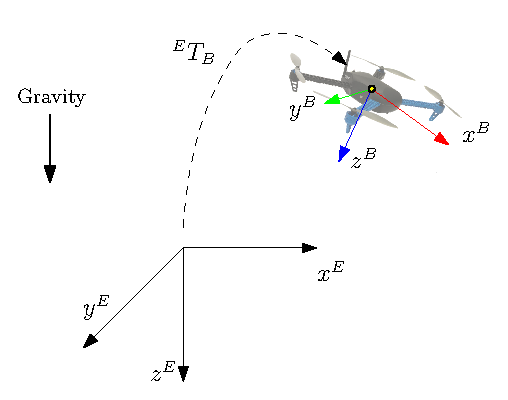
\includegraphics[width=0.8\textwidth]{ref_frames.eps}
 \caption[Reference frames for modeling]{Earth-fixed reference frame,  body-fixed reference frame and the transformation between them.}
 \label{figure:refframes}
\end{figure}

\subsection{General assumptions}

The analysis of this system is pretty complex. In order to simplify the derivation of the model some assumptions are made and some non linearities are disregarded. \\ 

\noindent
When a rotor translates horizontally through the air, the advancing blade has a higher absolute tip velocity and will generate more lift than the retreating blade. The mismatch in lift generates an overall moment on the rotor disk in the direction of the apparent wind causing the blade to flap as shown in figure \ref{figure:refframes} and the generated thrust is inclined respect to the rotor axis. This effect, called \textit{Blade Flapping} is not included in the derived model.

\begin{figure}[h]
\centering
 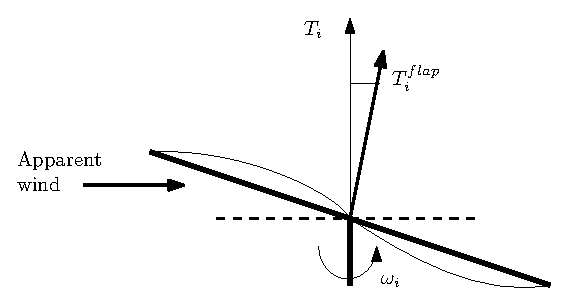
\includegraphics[width=0.7\textwidth]{bladeflap.eps}
 \caption[Blade flapping]{Blade flapping effect. $T_i$ is the ideal vertical thrust while $T_i^{flap}$ is the real thrust vector}
 \label{figure:refframes}
\end{figure}
A second disregarded non linear effect is the \textit{Total Thrust Variation in Translational Flight} \cite{Huang2009}. The analysis of this phenomenon is quite complex and it is described by a  qualitative explanation. When a rotor translates in air, it suffers form apparent wind and an increase of air flux through the blades. This leads to an increase of lift and thrust by the rotor.\par
Moreover, viscous friction experienced by the robot when it moves is negligible at small velocities. The robot can be also considered as a rigid body since there are no significant strains and forces applied which may deform the structure. \\*

\noindent
To summarize, the following assumption are made:
\begin{itemize}
\item Blade Flapping is not considered
\item Thrust Variation in Translational Flight is disregarded
\item Viscous friction (drag) is neglected
\item The robot is considered as a rigid body
\item Motor dynamics are managed internally by the board and not included in the model
\end{itemize}

\section{Transformation matrices}
\label{sec:trasfmatrix}
This Section introduces some mathematical tools necessary to develop a full dynamical model for the quadrotor system. Moreover I will present here the conventions used for representing angles and rotations and the derivation of the matrices involved. \\ 

\noindent
In Section \ref{sec:refframes} I introduced ${}^ET_B$ as the transformation matrix of $\Re^B$ with respect to $\Re^E$. In particular ${}^ET_B$ is a $4\times4$ matrix and has a fixed structure \cite{Khalil2004}: \begin{equation}
{}^ET_B = \begin{bmatrix}
{}^ER_B&&{}^EP_B\\
O_3^T&&1
\end{bmatrix}
\label{eq:transdef}
\end{equation}
in this definition we can see three different terms. ${}^ER_B$ is the rotation matrix of frame $\Re^B$ with respect to $\Re^B$; ${}^EP_B$ = $\begin{bmatrix}x\\y\\z\end{bmatrix}$ is the position of the center of mass of the robot respect to the Earth frame and $O_3$ = $\begin{bmatrix}0\\0\\0\end{bmatrix}$. 

\subsection*{Rotation matrix and angles}

Every rotation in 3D space can be defined by 3 successive rotations about 3 principal axis; we can define separately each rotation matrix about each axis and the multiply them.\\ 

\noindent
Each Right-Hand rotation about a particular axis is defined by a positive angle \cite{Blanco2010} from earth to body frame and the following definitions are true:

\begin{equation}
R_x(\phi) = \begin{bmatrix} 1 & 0            & 0 \\
							  0 & \cos(\theta) & \sin(\theta)\\
                              0 & -\sin(\theta) &  \cos(\theta) 
\end{bmatrix}
\end{equation}

\begin{equation}
R_y(\theta) = \begin{bmatrix} \cos(\theta)  & 0 & \sin(\theta) \\
							  0 & 		      1 &   0\\
                              -\sin(\theta) &  0 &  \cos(\theta) 
\end{bmatrix}
\end{equation}

\begin{equation}
R_z(\psi) = \begin{bmatrix} \cos(\psi)  & -\sin(\psi) &0 \\
							\sin(\psi) & \cos(\psi) &0\\
                              0         & 0          &1 
\end{bmatrix}
\end{equation}
The general rotation matrix can be obtained by multiplying elemantary rotations, but please note that the order is important.\\

\noindent
The most common sequence associated with the name \textit{Euler angles} is $(z, x, z)$ or ${}^ER_B = R_z(\phi)R_x(\theta)R_z(\psi)$.\\ 

\noindent
There is however a more suitable sequence with fits our case. The angles associated with the sequence $(x, y, z)$ are sometimes called \textit{Cardan angles} or \textit{Tait-Bryan angles}. Commonly used in aerospace where $\phi$, $\theta$, and $\psi$ are known respectively as\textbf{ roll}, \textbf{pitch}, and \textbf{yaw}. These angles describe a vehicle whose forward direction is along the positive body-fixed x-axis and the body-fixed z axis downward, like in the case of the quadrotor (see Section \ref{sec:refframes}). In such configuration, the home position $\begin{bmatrix}\phi\\ \theta \\ \psi \end{bmatrix} = \begin{bmatrix}0\\ 0 \\ 0 \end{bmatrix}$ , is flat and level pointing forward along the world x axis. The non intuitive downward pointing z axis is chosen in order to make a positive change in $\theta$ correspond to pitching upward \cite{Diebel2006}. \\

\noindent
Having said that, the multiplication order used is $(x , y , z)$. Developing the calculations, the general rotation matrix becomes:\begin{equation}
{}^ER_B = R_x(\phi)R_y(\theta)R_z(\psi) = \begin{bmatrix} 
c_\theta c_\psi && s_\phi s_\theta c_\psi - c_\phi s _\psi &&  c_\phi s_\theta c_\psi + s_\phi c _\psi \\
c_\theta s_\psi&& s_\phi s_\theta s_\psi + c_\phi c _\psi && c_\phi s_\theta  s_\psi - s_\phi c _\psi \\
-s_\theta && c_\theta s_\phi  &&  c_\theta c_\phi 
\end{bmatrix}
\label{eq:rotmatrix}
\end{equation}where $c = cos$ and $s = sin$ for simplicity, Moreover, the following limits are true by definition: \begin{itemize}
\item $ -\pi < \phi < \pi$
\item $ -\pi/2 < \theta < \pi/2$
\item $ -\pi < \psi < \pi$
\end{itemize}
while the following shows the transformation from the derivative of the Euler angles to the angular velocity in the body frame\cite{Friis2009}:
\begin{equation}
W = \begin{bmatrix} 
1 && 0 && -s_\theta\\
0 && c_\phi && c_\theta s_\phi \\
0 && -s_\phi && c_\theta c_\phi
\end{bmatrix}
\end{equation}
Please also note that ${}^ER_B$ is an orthonormal 3x3 matrix so its inverse it is equal to its transpose \cite{Khalil2004}, hence $({}^ER_B)^{-1} = ({}^ER_B)^{T}$ = ${}^BR_E$.

\section{Propulsion and controls}
\label{sec:propulsion}

The four motors installed are responsible of the propulsion of the quadcopter. Each rotor-motor couple rotates with an angular velocity $\omega_i$ and generates: an upward lifting force $f_i$ parallel to the body z axis $z^B$ and a reaction torque $\tau_r$. This quantities approximated by a linear model where: \begin{equation}
f_i = k \omega_i ^ 2
\label{eq:fi}
\end{equation}
\begin{equation}
\tau_i = k_d \omega_i ^ 2
\label{eq:taui}
\end{equation}
$k$ and $k_d$ are positive constants depending on atmospheric conditions and blade geometry (\cite{Mahony2012} and \cite{Falchi2014}). This constants can be identified through dynamical tests but in this case they are provided in the autopilot configuration file.\\

\begin{figure}[h]
\centering
 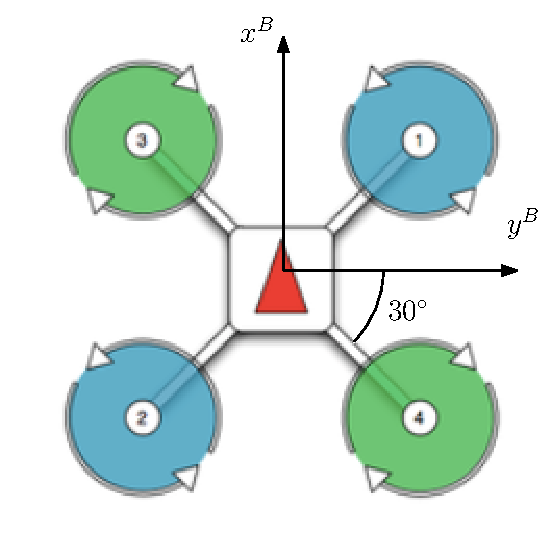
\includegraphics[width=0.5\textwidth]{top_iris.eps}
 \caption[Motor rotations]{Motor labeling and spinning}
 \label{figure:motorspin}
\end{figure}

\noindent
The total thrust $T$ acting on the robot's center of mass, parallel to $z^B$ and directed upwards is:
\begin{equation}
\boldsymbol{T^B}=\begin{bmatrix}0\\0\\\sum_{i=1}^{4}f_i
\end{bmatrix}
\label{eq:T}
\end{equation}
while the total moments
\begin{equation}
\tau_\phi = \sum_{i=1}^{4}d_1\sin(\alpha_i) f_i
\label{eq:tauph}
\end{equation}
\begin{equation}
\tau_\theta = -\sum_{i=1}^{4}d_i\cos(\alpha_i) f_i
\label{eq:tauth}
\end{equation}
\begin{equation}
\tau_\psi = \sum_{i=1}^{4}\sigma_i\cos(\alpha_i) \tau_i
\label{eq:taups}
\end{equation}
where $f_i$ and k are defined in \eqref{eq:fi}; $\tau_i$ and $k_d$ in \eqref{eq:taui}; $d_i$ is the distance from the center of the rotor to the center of mass; $\sigma_i$ is positive if $\omega_i$ is positive and negative otherwise; $\alpha_i$ is the angle between the vector going from the center of mass to the \textit{i-th} motor and $y^B$ ($30^\circ$ for IRIS).\\

\noindent
By rearranging \eqref{eq:tauph}, \eqref{eq:tauth} and \eqref{eq:taups} in matrix form:
\begin{equation}
\begin{bmatrix}
T^B\\\tau_\phi\\\tau_\theta\\\tau_\psi
\end{bmatrix} = \begin{bmatrix}
k&&k&&k&&k\\
k d_i \sin(30)&&-k d_i \sin(30)k&& -d_i \sin(30)&&d_i \sin(30)\\
-k d_i \cos(30)&&-k d_i \cos(30)k&& d_i \cos(30)&&d_i \cos(30)\\
k_d&&-k_d&&-k_d&&k_d
\end{bmatrix} \begin{bmatrix}
\omega_1^2\\\omega_2^2\\\omega_3^2\\\omega_4^2
\end{bmatrix}
\label{eq:inputmix}
\end{equation}

\begin{equation}
\begin{bmatrix}
T^B\\\tau_\phi\\\tau_\theta\\\tau_\psi
\end{bmatrix} = H \begin{bmatrix}
\omega_1^2\\\omega_2^2\\\omega_3^2\\\omega_4^2
\end{bmatrix}
\label{eq:inputmixmatrix}
\end{equation}
where in this case $T^B$ is the value of the force directed through $z^B$, $\tau_\phi$ is the torque along $x^B$, $\tau_\theta$ is the torque along $y^B$ and finally  $\tau_\psi$ is the torque along $z^B$. The force $T^B$ is responsible of the translation or the body frame while the three torques generate rotations in each principal axis.

Figure \ref{figure:motorspin} shows how motors are labeled in IRIS and the respective direction of rotation while \ref{figure:forces} is a diagram with the applied forces on the rigid body.

\begin{figure}[h]
\centering
 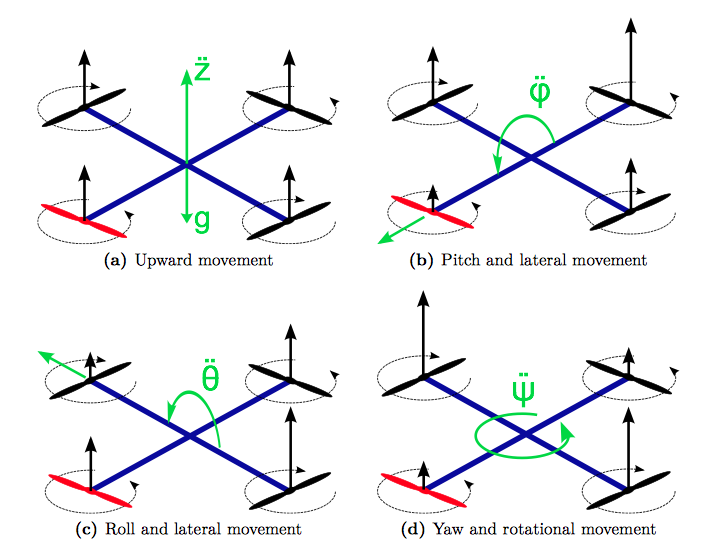
\includegraphics[width=0.7\textwidth]{forces.png}
 \caption[Quad dynamics]{Dynamics of the copter. Assume that x axis points towards the red propeller for simplicity, black arrows are the generated forces $f_i$ from aerodynamics. Green arrows represent forces and torques generated combining the rotational speed of the propellers.}
 \label{figure:forces}
\end{figure}


\section{Complete model}

Equation \eqref{eq:inputmix} shows the relation between the squared velocity of each rotor and the generated force and torques  . Hence the problem can be split in two parts, aerodynamics and equations of motion. Therefore, \textbf{the model is defined as a rigid body on which one external force $T^B$ and three external torques $[\tau_\phi ; \tau_\theta ; \tau_\psi]$ are applied.} Those external perturbations are calculated in Section \ref{sec:propulsion} and they correspond to the aerodynamic propulsion of the blades. 

\subsection{Rigid body equations}

In order to develop the full dynamical model, the control signals must be introduced. Let us define $U$ as a 4-element control vector, then the following is true by definition:
\begin{equation}
\textbf{U} = \begin{bmatrix}
T^B\\\tau_\phi \\ \tau_\theta \\ \tau_\psi
\end{bmatrix}
\label{eq:inputs}
\end{equation}
Let us also approximate the inertia of the blades equal to zero for simplicity as in \cite{Vendittelli}. We can define the following quantities:\begin{itemize}
\item $\boldsymbol{r}$ = $\begin{bmatrix} x\\y\\z\end{bmatrix}$ position of the robot in Earth frame.
\item $\boldsymbol{\eta}$ = $\begin{bmatrix} \phi\\\theta\\\psi\end{bmatrix}$ attitude of the quadcopter respect to earth frame (roll, pitch, yaw) presented in Section \ref{sec:trasfmatrix}.
\item $\boldsymbol{\Omega}$ = $\begin{bmatrix} p\\q\\r\end{bmatrix}$ body angular speed respect to each axis in body frame.
\item ${}^ER_B = R(\eta)$ rotation matrix encoding body attitude defined in Section \ref{sec:trasfmatrix} such that $\boldsymbol{x^E} =  R(\eta) \boldsymbol{x^B}$.

\item $W = W(\eta)$ Euler angle rate matrix defined in Section \ref{sec:trasfmatrix} relating $\boldsymbol{\Omega}$ with $\dot{\boldsymbol{\eta}}$ 
\end{itemize}
The dynamics of the quadcopter can be described by the use of Newton-Euler cardinal equation for motion of a general 6 DOF rigid body suffering from an external force and torque. The four equations for the undergoing motion are defined as the following:

\begin{align}
\label{eq:rigidb1}
\boldsymbol{\dot{r}}& = \boldsymbol{v}\\ \label{eq:rigidb2}
m\boldsymbol{\dot{v}}& = \boldsymbol{F}\\ 
\label{eq:rigidb3}
\dot{R}& = R\Omega_\times\\ 
\label{eq:rigidb4}
I\boldsymbol{\dot{\Omega}}& = -\boldsymbol{\Omega} \times I\boldsymbol{\Omega} + \boldsymbol{\tau}
\end{align}
\noindent
where the vector $\boldsymbol{F}$ is the resultant of all the external forces applied on the rigid body's center of mass and $\boldsymbol{\tau}$ is the total torque acting on the body. $\Omega_\times$ is a $3\times3$ skew symmetric matrix such that $\Omega_\times \boldsymbol{v} = \boldsymbol{\Omega} \times \boldsymbol{v}$ for the vector cross product $\times$ and any vector $\boldsymbol{v}$ \cite{Mahony2012}. The inertia matrix is diagonal of the form
\begin{equation}
	I=\begin{bmatrix}
	I_{xx}&&0&&0\\0&&I_{yy}&&0\\0&&0&&I_{zz}
	\end{bmatrix}
\end{equation}
due to the symmetries of the body about principal axis while $m$ is the total mass of the robot.

\paragraph{Equations for translation}

Since viscosity in air is not considered, the total forces acting on the robot are the gravity $m\boldsymbol{g}$ and the thrust generated by the rotors $\boldsymbol{T^B}$ calculated in equation \eqref{eq:T}. \\

\noindent
Let us define $U_1 = T^B$ meaning the first element of the control vector $U$ introduced in \eqref{eq:inputs} where $T^B$ is the module of the thrust directed along $z^B$ (see equation \eqref{eq:inputmix}).
As consequence \eqref{eq:rigidb2} can be written as follows:
\vspace{1ex}
\begin{equation}
\vspace{1ex}
\boldsymbol{\dot{v}} = \frac{1}{m}\left(\begin{bmatrix}0\\0\\mg\end{bmatrix}^E + R\begin{bmatrix}0\\0\\U_1\end{bmatrix}^B\right)
\label{eq:rigidb2new}
\end{equation}
\textbf{Note:} the first column vector in equation \eqref{eq:rigidb2new} is the gravity force and is directed along $z^E$ on its positive direction (downwards). The second column vector is the thrust in body frame which is along $z^B$ pointing to its positive direction. The multiplication with the rotation matrix $R$ rotates the thrust vector expressing in in earth frame since $\boldsymbol{v}$ must be expressed in earth frame.\\

\noindent
\paragraph{Equations for rotation}
The total torques acting on the robot are those originated by the commanding maneuvers calculated in equation \eqref{eq:inputmix} and the gyroscopical effect induced by the rotating blades. \par The gyroscopic torques can me neglected because the mass of the blades is very low, then the total torque applied on the rigid body is the one originated by the lifting forces and we have that $\boldsymbol{\tau} = \begin{bmatrix}
\tau_\phi\\\tau_\theta\\\tau_\psi
\end{bmatrix}$. Those values are namely the second, the third and the forth elements of the control vector $U$ hence equation \eqref{eq:rigidb4} becomes:
\vspace{1ex}
\begin{equation}
\vspace{1ex}
\boldsymbol{\dot{\Omega}} =I^{-1}\left(\begin{bmatrix}
U_2\\U_2\\U_4
\end{bmatrix} -\boldsymbol{\Omega} \times I\boldsymbol{\Omega}\right)
\label{eq:rigidb4new}
\end{equation}
where it has this simple form due to the assumption of null gyroscopic effects.\\

\noindent
Moreover, equation \eqref{eq:rigidb3} can be substituted by the explicit relation between angle rates in earth and in body frame through the matrix $W$ \cite{Kendoul2007}. Thus, equation \eqref{eq:rigidb3} is replaced by:
\vspace{1ex}
\begin{equation}
\vspace{1ex}
\boldsymbol{\dot{\eta}} = W\boldsymbol{\Omega}
\label{eq:rigidb3new}
\end{equation}
where, for recalling, $\boldsymbol{\Omega}$ is the angular velocity vector in body frame.

\subsection*{Full non linear model}
Expanding equations \eqref{eq:rigidb1}, \eqref{eq:rigidb2new}, \eqref{eq:rigidb3new} and \eqref{eq:rigidb4new} we obtain the full mathematical model represented by the following differential equations:
\vspace{2ex}
\begin{equation}
\vspace{2ex}
\left\lbrace
	\begin{aligned}
		\dot{x}& = v_x \\
		\dot{y}& = v_y \\
		\dot{z}& = v_z \\
		\dot{v_x}& = -\frac{U_1}{m}(\cos(\phi)\sin(\theta)\cos(\psi) + \sin(\phi)\sin(\psi) \\
		\dot{v_y}& = -\frac{U_1}{m}(\cos(\phi)\sin(\theta)\sin(\psi) + \sin(\phi)\cos(\psi) \\
		\dot{v_z}& = g - \frac{U_1}{m}(\cos(\phi)\cos(\theta) \\
        \dot{\phi}& = p - r \sin(\theta) \\
        \dot{\theta}& = q \cos(\phi) + r\cos(\theta) \sin(\phi) \\
        \dot{\psi}& = r \cos(\phi) \cos(\theta) - q \sin(\phi)\\
        \dot{p}& =\frac{1}{I_{xx}}(U_2 + qr(I_{yy} - I_{zz})) \\
        \dot{q}& =\frac{1}{I_{yy}}(U_3 + pr(I_{zz} - I_{xx})) \\
        \dot{r}& =\frac{1}{I_{zz}}(U_4 + pq(I_{xx} - I_{yy})) \\
     \end{aligned}
     \right.
\label{eq:mathfullmodel}
\end{equation}
I want to stress that this model does not take into account factors such as aerodynamic drag, ground effect, blade-flapping, gyroscopic effects or advanced aerodynamics phenomenons. Even with this approximations, this model is the most used in the research because it assures good precision.

\subsubsection*{Simplified model}
Further simplifications can be applied, let us consider the quadrotor in the flat position and now assume that the variation of roll and pitch angles are reasonably small. This is a logical assumption since the quadcopter is designed to fly around such configuration; we can assume that $\phi \approx 0$ and $\theta \approx 0$ and the matrix $W$ becomes an identity matrix as consequence. Therefore under those conditions we have that $\boldsymbol{\dot{\eta}} = \boldsymbol{\Omega}$ and the model is:

\vspace{2ex}
\begin{equation}
\vspace{2ex}
\left\lbrace
	\begin{aligned}
		\dot{x}& = v_x \\
		\dot{y}& = v_y \\
		\dot{z}& = v_z \\
		\dot{v_x}& = -\frac{U_1}{m}(\cos(\phi)\sin(\theta)\cos(\psi) + \sin(\phi)\sin(\psi) \\
		\dot{v_y}& = -\frac{U_1}{m}(\cos(\phi)\sin(\theta)\sin(\psi) + \sin(\phi)\cos(\psi) \\
		\dot{v_z}& = g - \frac{U_1}{m}(\cos(\phi)\cos(\theta) \\
        \dot{\phi}& = p \\
        \dot{\theta}& = q  \\
        \dot{\psi}& = r \\
        \dot{p}& =\frac{U_2}{I_{xx}} \\
        \dot{q}& =\frac{U_3}{I_{yy}} \\
        \dot{r}& =\frac{U_4}{I_{zz}} \\
     \end{aligned}
     \right.
\label{eq:mathlinlmodel}
\end{equation}

\noindent
Please note that only the rotational dynamics are simplified. This model, even with the various assumptions and the linearization, is often used to try simple control algorithm and design linear controllers. In our case it is useful since this project do not include the study on aggressive maneuvering or high velocity motions, the small angle variation for roll and pitch is a valid assumption in fact thi model is used to design controllers for hovering. 

\begin{table}[h]
\centering
\begin{tabular}{c c r}
\hline
$m$ & total mass of the robot & $1.308$ Kg \\
$I_xx$& inertia for the x axis& $0.0018$ Kg $m^2$ \\
$I_yy$& inertia for the y axis& $0.0012$ Kg $m^2$ \\
$I_zz$& inertia for the z axis& $0.0027$ Kg $m^2$ \\ \hline
$k$   & thrust coefficient & $0.1$ \\
$k_d$ & drag coefficient & $ 0.1$ \\
\end{tabular}
\caption{IRIS parameters. The moment of inertia are taken from the autopilot parameters file while the aerodynamic coefficients are taken from the blade technical sheet.}
\end{table}















